% ch-firstrun.tex -- the first calculation, start to finish
\chapter{Your first calculation}
\label{ch:firstrun}

This chapter runs one case from beginning to end, looks at what came out, and
then changes one thing at a time so that you can see which part of the input
file controls which part of the answer. It assumes you have built Yuzen as in
\cref{ch:installation}.

\section{Running a case}
\label{sec:firstrun:run}

A run takes one argument, the input file:

\begin{shell}
cd <repository root>
mkdir -p run1 && cd run1
../build/bin/yuzen ../cases/tutorial_1d.toml
\end{shell}

The input file may be given by any path, relative or absolute, with spaces or
non-ASCII characters in it. Besides it the solver knows three options:
\code{--check-input FILE} reads and checks the file and runs nothing
(\cref{sec:inputformat:unknown}), \code{--help} prints the usage and
\code{--version} the version. Anything else --- no argument, two input files,
an unknown option --- prints the usage on standard error and ends with exit
code 1, as does an input file that is missing, a directory or unreadable.
\Cref{tab:exitcodes} lists the exit codes.

It prints a banner, the version and the OpenMP thread count, reads the input,
checks it for consistency, creates the result directory and starts stepping.
The result directory is named after the \key{JobName} key in the input file ---
not after the input file --- so this run produces \file{tutorial\_1d/}. Every
case under \file{cases/} sets \key{JobName} to its own file name, so the
result directory is named after the case it came from.

\begin{note}[Run in a scratch directory]
  Output is written relative to the working directory, so run from wherever you
  want the results. \file{tools/run\_case.sh} does exactly that, and fixes the
  thread count and keeps the log as well (\cref{sec:env:tools}):
  \begin{shell}
./tools/run_case.sh cases/leveling_1d_reg.toml runs/reg 1
  \end{shell}
\end{note}

The case used here, \file{cases/tutorial\_1d.toml}, is a 1-D well-mixed film:
\SI{1}{\milli\metre} wide, \SI{300}{} cells, a \SI{10}{\micro\metre} height
scale, capillary leveling and Marangoni stress on, evaporation on, running to
\SI{0.5}{\second}. It takes a few seconds.

\section{What came out}
\label{sec:firstrun:output}

\begin{plain}
tutorial_1d/
  tutorial_1d.toml        a copy of the input, so the directory is self-describing
  JobInfo.txt             version, machine, linear-solver backends, start and end time
  Warnings.txt            warnings; zero-length if there were none
  FatalErrors.txt         why the run aborted; zero-length if it did not
  field00000.dat ...      the field, as tab-separated text (also the restart format)
  field00000.vts ...      the same field as VTK structured grid
  field00000.state ...    what a restart needs beyond the field (time, step, totals)
  tutorial_1d.pvd         ParaView time series pointing at the .vts files
  History.dat             volume, mean concentration, extrema, conservation error
  CalcInfo.dat            per-output-interval solver diagnostics
\end{plain}

The terminal and the text files at the top of the listing are worth reading
first, in this order.

\paragraph{The terminal} carries the run log: it goes to standard output and is
not written to any file in the result directory. What you saw scroll past opens
with what the solver built from your input --- the linear-solver backend and
the convection scheme of each equation, the grid, the scales used to non-dimensionalize the
problem ($L_0$, $H_0$, $T_0$, $U_0$, under \code{Scaling factors}) and the
dimensionless groups derived from them, the model --- and then becomes the
progress log. A
dot is one time step, \code{dt+} and \code{dt-} mark the adaptive step growing
and shrinking, and \code{Field file $n$, Time = $\dots$} marks each field
written. The run ends with the termination message, and it is the first thing
to check:

\begin{plain}
############## Time reached to the EndTime. #############
Field file 5, Time = 1.606806e-05
Largest Courant number of Numerics.Convection.Height = "Koren": 0.000469

############## Program normally terminated. #############
\end{plain}

There are three normal endings --- \code{Time reached to the EndTime.},
\code{Dry out.} and \code{Steady state.} --- and they mean quite different
things about your case. \Cref{sec:convergence:termination} explains each, and
in particular why a run that reports \code{Steady state.} after a dozen steps is
usually telling you something about the criterion rather than about the physics.

To keep the log, redirect it yourself --- \code{yuzen case.toml > run.log} ---
or use \file{tools/run\_case.sh}, which does the redirection for you and leaves
everything the terminal would have shown in \file{stdout.txt} in the run
directory.

To stop a run early, press Ctrl-C once: the step in progress finishes, the
state reached is written as a field file with its \file{.state}, and the run
ends with \code{Program stopped by SIGINT; its output is complete.} That file
can be restarted from (\cref{sec:firstrun:restart}) and the continued run is
the one that was not stopped, to the bit. A second Ctrl-C ends the process at
once. \Cref{sec:output:failures} has the details, and what happens on a full
disk.

\paragraph{\file{JobInfo.txt}} records the version, the compiler, the machine,
the start and end times, and one section derived from your input: the model and
the linear-solver backend that each equation actually used
(\cref{sec:output:jobinfo}). If a result looks wrong by orders of magnitude,
the scales to check --- $L_0$, $T_0$ and $U_0$ --- are in the run log, not here
(\cref{sec:governing:scales}).

\paragraph{\file{Warnings.txt}} always exists and carries no banner, so it is
\textbf{zero-length exactly when no warning was raised}. Anything in it is a
real message.

\paragraph{\file{FatalErrors.txt}} exists too, and is likewise zero-length
unless the run aborted. When it does abort, the reason is written here
\emph{and} to standard error, so the message is in the result directory and on
the terminal at once. The one case with no file to read is an input the solver
rejects: that happens before the result directory is made, so the message is on
standard error only (\cref{sec:output:warnings}).

\section{Reading the field files}
\label{sec:firstrun:fields}

\file{field00000.dat} is tab-separated text with a one-line header. In 1-D:

\begin{plain}
xx[mm]  HS[um]  Ux[m/s]  CC[-]  HH[um]  SS[um]
-5.00000000000000111e-01  5.00000000000000000e+00  0.0 ...
\end{plain}

\begin{yzntable}{Columns of \file{field*.dat}\label{tab:fieldcols}}{@{}L{0.09\textwidth} L{0.13\textwidth} L{0.70\textwidth}@{}}
\textsf{\bfseries 1-D} & \textsf{\bfseries 2-D} & \textsf{\bfseries Meaning}\\ \midrule
\code{xx} & \code{xx}, \code{yy} & in-plane coordinate, in \si{\milli\metre} \\
\code{HS} & \code{HS}            & free-surface height, $h + s$, in \si{\micro\metre} \\
\code{Ux} & \code{Ux}, \code{Uy} & in-plane velocity, the mixed velocity of all active terms, in \si{\metre\per\second} \\
\code{CC} & \code{CC}            & solute concentration, a mass fraction \\
\code{HH} & \code{HH}            & film thickness $h$, in \si{\micro\metre} \\
\code{SS} & \code{SS}            & substrate height $s$, in \si{\micro\metre} \\
\end{yzntable}

The units above are what you get with \key{Output.Dimensioned} at its default
\val{true}; with \val{false} every column is non-dimensional. Note that the
in-plane and out-of-plane lengths are \emph{not} in the same unit, which is why
the sample line above reads $-0.5$ for a point \SI{0.5}{\milli\metre} from the
center and $5.0$ for a film \SI{5}{\micro\metre} thick.

\begin{warn}[\code{HS} is the free surface, \code{HH} is the thickness]
  The second column is $h+s$, not $h$. \Cref{fig:film-geometry} shows which is
  which. The concentration is the fourth column, not the last one.
\end{warn}

\begin{figure}[tbp]
  \centering
  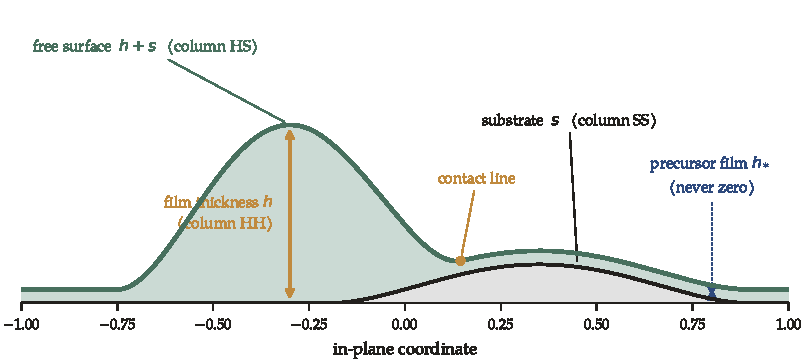
\includegraphics[width=\textwidth]{figures/film-geometry.pdf}
  \caption{The three height columns of \file{field*.dat}, on a droplet sitting
    on a precursor film over a substrate feature. \code{SS} is the substrate
    $s$, \code{HS} is the free surface $h+s$ --- the profile you would see ---
    and \code{HH} is the film thickness $h$ between them. Over a flat substrate
    \code{HS} and \code{HH} coincide and the distinction is invisible; over
    topography they are the difference between the surface you would see and
    the layer of liquid there is. The precursor film $h_*$, set by
    \key{Initial.\bk SurfaceShape.\bk PrecursorRatio}, is the floor below which
    \code{HH} never falls, so the contact line is where the free surface meets
    it rather than a point of zero thickness (\cref{ch:wetting}).
    \label{fig:film-geometry}}
\end{figure}

Whether these numbers are dimensional or dimensionless is set by
\key{Output.Dimensioned}. The values are written with 18 significant digits
regardless, because this same file is the ASCII restart format: at the default
six digits, passing the height through a second difference (dividing by
$\Delta x^2$) corrupts the pressure --- on a contact-line mesh with $\Delta x =
\SI{0.3}{\micro\metre}$, output precision alone shifted the pressure by a few
percent and the velocity derived from it by three orders of magnitude.

For a quick look at the shape, any plotting tool will do:

\begin{shell}
gnuplot -p -e 'plot "tutorial_1d/field00004.dat" u 1:2 w l title "free surface"'
\end{shell}

\section{Viewing in ParaView}
\label{sec:firstrun:paraview}

Open \file{tutorial\_1d/tutorial\_1d.pvd}. It is a collection pointing at the
\file{.vts} files with their time stamps, so ParaView gets the whole time
series with the correct times in one step --- not a numbered sequence it has to
guess at. Set
\key{Output.FieldData.VTKFile} to \val{false} if you do not want the VTK files
at all; \key{NeutralFile} controls the text ones independently.

\section{Changing one thing at a time}
\label{sec:firstrun:changing}

Copy the case and edit it. The following changes are, in rough order, the ones
worth making first.

\paragraph{Run longer or shorter.} \key{Numerics.EndTime}, in seconds. Note
that it defaults to \val{0}, which stops the run after a single step rather
than meaning ``no limit'' --- so always set it.

\paragraph{Write more often.} \key{Output.\bk FieldData.\bk TimeInterval} governs the
fields, \key{Output.\bk GeneralHistory.\bk TimeInterval} the scalar history and
\key{Output.\bk CalcInfo.\bk TimeInterval} the solver diagnostics. They are independent;
history and diagnostics are cheap, so it is normal to write them ten to a
hundred times more often than the fields.

\paragraph{Refine the mesh.} \key{Grid.Nx}, counting interior cells only.
Refinement is not free in an unobvious way: the Newton correction cannot fall
below a floor, and the part of it that comes from terms formed as a product
with their matrix entries grows with the step and as the mesh is refined
(\cref{sec:convergence:floor}). If a refined case suddenly becomes very slow,
read \cref{sec:convergence:absolute} before changing anything else.

\paragraph{Turn a physics term on or off.} Every term under \key{Physics} has
its own \key{Enable}. In \file{tutorial\bk\_1d.toml}, vertical gravity,
in-plane gravity, the centrifugal term and the source are off, and
\file{cases/\bk allphys\_1d\_reg.toml} is the same case with everything on.

\paragraph{Make it dry.} \key{Physics.Evaporation.Coef} sets the evaporation
velocity in \si{\metre\per\second}; it feeds both $\Ev$ and $\Pen$. Watch
\code{AveC} in \file{History.dat} rise as the solvent leaves. With the
viscosity exponent at 10, as in this case, a concentration change of 0.1
multiplies the viscosity by $e$, and the film visibly stops flowing --- that
coupling is the most strongly non-linear thing in the solver
(\cref{sec:conc:properties}).

\paragraph{Add a contact line.} Enable \key{Physics.DisjoiningPressure} and set
\key{ContactAngle}, \key{ExponentN}, \key{ExponentM} and
\key{Initial.SurfaceShape.PrecursorRatio}. Do not do this without reading
\cref{sec:wetting:sizing} first: the mesh and the droplet height are not free
choices once you have named a contact angle, and a case that violates the two
sizing rules produces an answer that looks plausible and has the wrong angle in
it.

\section{Restarting}
\label{sec:firstrun:restart}

Because \file{field*.dat} is also the restart format, any output can be a
starting point. Point \key{Restart} at the file and enable it:

\begin{toml}
[Restart]
Enable      = true
ASCII       = true
FileName    = "tutorial_1d/field00005.dat"
RestartTime = 0.501237
FileIndex   = 6
\end{toml}

and raise \key{Numerics.EndTime}, which is absolute, past \key{RestartTime}.
\key{RestartTime} is the time of that file as \file{tutorial\_1d.pvd} lists
it: a field is written at the step nearest its scheduled time, not exactly on
it. Given that time, the run reads \file{field00005.state} beside the field
file as well and continues exactly as the uninterrupted run would have
(\cref{sec:ref-numerics:restart}); the run log says
\code{continuing exactly from tutorial\_1d/field00005.state}. Given another
time, it takes the field alone and says so.

\key{FileName} is resolved relative to the \textbf{working directory you launch
the solver from}, not relative to the result directory. The file written by the
run above landed in \file{tutorial\_1d/}, so from the same directory you ran in,
the path has to carry that prefix; a bare \file{field00005.dat} would only work
if you ran from inside \file{tutorial\_1d/} --- which would also be where the
new run tried to write its own results.

The shape in \key{Initial.SurfaceShape} is then read but not used. This is also
how an analytically constructed initial state gets in: \file{cases/eq/} and
the \file{cases/wet\_*.toml} cases start from equilibrium droplets built by
\file{tools/make\_equilibrium\_1d.py}, precisely so that the run does not begin
with a spurious velocity at the contact line. \Cref{ch:ref-numerics} documents
the keys and \cref{sec:wetting:equilibrium} the construction.

\section{Comparing two runs}
\label{sec:firstrun:compare}

\begin{shell}
./tools/run_case.sh cases/leveling_1d_reg.toml runs/reg_th1 1
./tools/run_case.sh cases/leveling_1d_reg.toml runs/reg_th2 2
python3 tools/compare.py runs/reg_th1 runs/reg_th2
\end{shell}

\file{tools/compare.py} reports, column by column, the largest difference
divided by the scale of that column, in \file{History.dat}, in
\file{CalcInfo.dat} and in the final \file{field*.dat}. For a pair of runs that
differ only in thread count the answer is \code{0.000e+00}, exactly, and this
is asserted rather than hoped for (\cref{sec:verification:linalg}). It is the
right tool to reach for after changing the solver: if the number is not zero,
you changed the numerics, not just the code.

The four solver-diagnostic columns of \file{CalcInfo.dat} --- \code{NK\_iter},
\code{NK\_resid}, \code{BCG\_iter} and \code{BCG\_resid} --- are held out of
that verdict and, when they differ, reported separately on the line of
\file{CalcInfo.dat}, as the largest
difference-over-column-scale among them. They say how the answer was reached
rather than what it is, so they may legitimately move; do not read that second
number as a total iteration count.
